\documentclass[preprint,12pt]{elsarticle}
% \documentclass[draft,12pt]{elsarticle}

\usepackage{hyperref}
\usepackage{graphicx}
\usepackage{subcaption}
\usepackage{amssymb}
\usepackage{amsmath}
\usepackage{multirow}
\usepackage{relsize}
\usepackage[utf8]{inputenc}
\usepackage{cleveref}
\usepackage{algorithm}
\usepackage[noend]{algpseudocode}
\usepackage[section]{placeins}
\usepackage{booktabs}
\usepackage{url}

% For the TODOs
\usepackage{xcolor}
\usepackage{xargs}
\usepackage[colorinlistoftodos,textsize=footnotesize]{todonotes}
\newcommand{\todoin}{\todo[inline]}
% from here: https://tex.stackexchange.com/questions/9796/how-to-add-todo-notes
\newcommandx{\unsure}[2][1=]{\todo[linecolor=red,backgroundcolor=red!25,bordercolor=red,#1]{#2}}
\newcommandx{\change}[2][1=]{\todo[linecolor=blue,backgroundcolor=blue!25,bordercolor=blue,#1]{#2}}
\newcommandx{\info}[2][1=]{\todo[linecolor=OliveGreen,backgroundcolor=OliveGreen!25,bordercolor=OliveGreen,#1]{#2}}

%Boldtype for greek symbols
\newcommand{\teng}[1]{\ensuremath{\boldsymbol{#1}}}
\newcommand{\ten}[1]{\ensuremath{\mathbf{#1}}}

\usepackage{lineno}
% \linenumbers

\journal{}

\begin{document}

\begin{frontmatter}

  \title{}
  \author[XXX]{Dinesh Adepu\corref{cor1}}
  \ead{d.dinesh@surrey.ac.uk}
  \author[University of Surrey]{Chuan Yu Wu}
  \ead{XXX}
\address[xxx]{xxx}

\cortext[cor1]{Corresponding author}


\begin{abstract}
\end{abstract}

\begin{keyword}
%% keywords here, in the form: keyword \sep keyword
{xxx}, {xxx}, {xxx}

%% MSC codes here, in the form: \MSC code \sep code
%% or \MSC[2008] code \sep code (2000 is the default)

\end{keyword}

\end{frontmatter}

% \linenumbers


\section{Governing equations}

\begin{equation}
  \label{eq:ce}
  \frac{d \rho}{d t} = - \rho \; \frac{\partial u_i}{\partial x_i},
\end{equation}
and conservation of linear momentum,
\begin{equation}
  \label{eq:me}
  \frac{d u_i}{d t} = \frac{1}{\rho} \; \frac{\partial \sigma_{ij}}{\partial x_j}
  + g_i,
\end{equation}
where $\rho$ is the density, $u_i$ is the $i$\textsuperscript{th} component of
the velocity field, $x_j$ is the $j$\textsuperscript{th} component of the
position vector, $g_i$ is the component of body force per unit mass and
$\sigma_{ij}$ is stress tensor.

The stress tensor is split into isotropic and deviatoric parts,
\begin{equation}
  \label{eq:stress_tensor_decomposition}
  \sigma_{ij} = - p \; \delta_{ij} + \sigma'_{ij},
\end{equation}
%
where $p$ is the pressure, $\delta_{ij}$ is the Kronecker delta function, and
$\sigma'_{ij}$ is the deviatoric stress.

The Jaumann's formulation for Hooke's stress provides us with the rate of
change of deviatoric stress,
\begin{equation}
  \label{eq:jaumann-stress-rate}
  \frac{d \sigma'_{ij}}{dt} = 2G (\dot{\epsilon}_{ij} - \frac{1}{3}
  \dot{\epsilon}_{kk} \delta_{ij}) + \sigma^{'}_{ik}  \Omega_{jk} +
  \Omega_{ik} \sigma^{'}_{kj},
\end{equation}
where $G$ is the shear modulus, $\dot{\epsilon}_{ij}$ is the strain rate tensor,
\begin{equation}
  \label{eq:strain-tensor}
  \dot{\epsilon}_{ij} = \frac{1}{2} \bigg(\frac{\partial u_i}{\partial x_j} +
  \frac{\partial u_j}{\partial x_i} \bigg),
\end{equation}
and $\Omega_{ij}$ is the rotation tensor,
\begin{equation}
  \label{eq:rotational-tensor}
  \Omega_{ij} = \frac{1}{2} \bigg(\frac{\partial u_i}{\partial x_j} -
  \frac{\partial u_j}{\partial x_i} \bigg).
\end{equation}

For a weakly-compressible or incompressible fluid, a viscous force is added:
\begin{equation}
  \label{eq:fluid-stress-decomposition}
  \sigma_{ij} = - p \delta_{ij} + 2 \eta \frac{\partial u_i}{\partial x_j}
\end{equation}
where $\eta$ is the kinematic viscosity of the fluid.

In both fluid and solid modelling the pressure is computed using an
isothermal equation of state, given as,
\begin{equation}
  \label{eq:pressure-equation}
  p = K \bigg(\frac{\rho}{\rho_{0}} - 1 \bigg),
\end{equation}
where $K = \rho_{0} c_0^2$ is the bulk modulus. Here, the constants $c_0$ and
$\rho_0$ are the reference speed of sound and density, respectively. For solids,
$c_0$ is computed as $\sqrt{\frac{E}{3 (1 - 2 \nu)\rho_{0}}}$, $\nu$ is the
Poisson ratio, $E$ is the Young's modulus.



\section{Smoothed Particle Hydrodynamics}
In the current section, we introduce the basics of smoothed particle
hydrodynamics. A fundamental overview of the discrete approximations of
function, derivative, and divergence is discussed.

\subsection{Function Approximation}
From the dirac delta function definition, the function value of a smooth
function $A$ defined over a domain $\Omega$ at point $x$ can be written as
\begin{equation}
  \label{eq:dirac_repr}
  A(\ten{x}) = \int_{\Omega}\> A(\ten{x}') \> \delta(\ten{x} - \ten{x}') \> d\ten{x}',
\end{equation}
where $\delta(\ten{x} - \ten{x}')$ is a Dirac-delta function with
\begin{equation}
  \label{eq:unity}
  \int_{\Omega}\> \delta(\ten{x}) \> d\ten{x} = 1.
\end{equation}
In SPH, the Dirac delta function is replaced with a compact, smooth function $W$,
chosen to be as an even function. The function value of $A$ at $\ten{x}$
interpolated with the smooth kernel $W$ is given by
\begin{equation}
  \label{eq:kernel_repr}
  A(\ten{x}) = \int_{\Omega}\> A(\ten{x}') \> W(\ten{x} - \ten{x}', h)  \> d\ten{x}' + O(h^2).
\end{equation}
Here, kernel $W$ satisfies the following conditions,
\begin{equation}
  \label{eq:unity}
  \int_{\Omega}\> W(\ten{x} - \ten{x}', h)  \> d\ten{x}' = 1.
\end{equation}

\begin{equation}
  \label{eq:kernel_delta}
  \lim_{h \to 0} W(\boldsymbol{x} - \boldsymbol{x}', h) = \delta(\boldsymbol{x} - \boldsymbol{x}', h).
\end{equation}
\begin{equation}
  \label{eq:compact_support}
  W(\boldsymbol{x} - \boldsymbol{x}', h) = 0 \>\>\>\>    \text{when}  \>\>\> |\boldsymbol{x} - \boldsymbol{x}'| > kh.
\end{equation}
Here k is a constant, which determines the the non-zero region $W$ for a point
at position vector $\boldsymbol{x}$. In the current work we have used Quintic
% spline in all our simulation cases. Quintic spline \parencite{Violeau16}, is
given as,
\begin{equation}
  \label{eq:quintic_spline}
  W(r, h) =
  \begin{cases}
    \sigma_5\left( (3-q)^5 - 6(2-q)^5 + 15(1-q)^5 \right), & \textrm{for} \ 0\leq q \leq 1,\\
    \sigma_5\left( (3-q)^5 - 6(2-q)^5 \right), & \textrm{for} \ 1 <  q \leq 2,\\
    \sigma_5 \ (3-q)^5 , & \textrm{for} \ 2 < q \leq 3,\\
    0, & \textrm{for} \ q>3,
  \end{cases}
\end{equation}
This type of interpolation leads to a 2nd order function accuracy
% \parencite{fatehi2011error}.

Assume that the domain is discretized into N particles with mass
$m_i$ and volume $\Delta v_i$, We have
\begin{equation}
  \label{eq:mass_repr}
  m_j = \Delta v_i \> \rho_i.
\end{equation}
Using \eqref{eq:mass_repr}, \eqref{eq:kernel_repr} is converted to
discrete form as follows
\begin{equation}
  \label{eq:discrete_form}
  A_i = \sum_{j \in \text{Neigh}(i)}\> \frac{m_j}{\rho_j} A_j\> W(\ten{x}_i - \ten{x}_j, h),
\end{equation}
where $A(\boldsymbol{x}_i) = A_i$ is the value of the field property of particle
i, similarly for $A_j$. Here, $\text{Neigh}(i)$ is the neighbours of particle $i$.

\subsection{Derivative Approximation}
% The discretized form of the derivative approximation~\parencite{Violeau16} is given
as,
\begin{equation}
  \label{intro:eq:derivative-discrete_form}
  \nabla A(\ten{x}_i) = \sum_j\> \frac{m_j}{\rho_j} A_j\> \nabla W(\ten{x}_i - \ten{x}_j, h).
\end{equation}

An alternative expression of the derivative approximation is derived by employing
density, i.e,
\begin{equation}
  \label{intro:eq:sph-continu-derivative-final}
  \nabla (A \rho^n) = n A \rho^{n - 1} \nabla \rho + \rho^n \nabla A,
\end{equation}
where $n$ is a real number. The new identity for the derivative of $A$ is
\begin{equation}
  \nabla A = \frac{1}{\rho^n} \left[ n A \rho^{n - 1} \nabla \rho + \rho^n \nabla A  \right],
\end{equation}
using \cref{eq:discrete_form,intro:eq:derivative-discrete_form}, the new
derivative approximation can be written as
\begin{equation}
  \label{intro:eq:derivative-discrete_form}
  \nabla A(\ten{x}_i) = \frac{1}{\rho^n(\ten{x}_i)} \sum\>
  m_j \left(A_j \rho^{n-1}(\ten{x}_j) - n A_i \rho^{n-1}(\ten{x}_i) \right)\> \nabla W(\ten{x}_i - \ten{x}_j, h).
\end{equation}
In the current work, we use a symmetric expression, with $n=-1$, resulting in
\begin{equation}
  \nabla A(\ten{x}_i) = \rho_i \sum_{j} m_j \left(\frac{A_i}{\rho_i^2} + \frac{A_j}{\rho_j^2}\right) \nabla W_{ij}.
\end{equation}
A symmetric gradient operator ensures equal and opposite forces acting on the
particles.


\subsection{Divergence Approximation}
We now look at an SPH approximation of the divergence operator. An approximation
of the divergence operator is used to discretize the \cref{eq:ce}. It is given
as,
\begin{equation}
  \label{intro:eq:discrete_derivative}
  \nabla \cdot \ten{v}_i = \sum\> \frac{m_j}{\rho_j} \ten{v}_j \cdot \nabla W(\ten{x}_i - \ten{x}_j, h).
\end{equation}
Similar to the derivative approximation, we utilize the following identity to approximate the divergence operator,
\begin{equation}
  \label{intro:eq:sph-continu-div-intermediate}
  \nabla \cdot (\ten{v} \rho^n) = \rho^n \nabla \cdot \ten{v} + n  \rho^{n - 1} \ten{v} \cdot \nabla \rho.
\end{equation}
In the current work, we employ expression for $n=1$. The discrete SPH approximation for $n=1$ is given as
\begin{equation}
  \label{intro:eq:sph-continu-div-final}
  \nabla \cdot \ten{v}(\ten{x}_i) = \frac{1}{\rho_i} \sum_{j} m_j \left(\ten{v}_j - \ten{v}_i\right) \cdot \nabla W_{ij}.
\end{equation}


\subsection{SPH Discretization}\label{sec:ctvf-sph-equations}

In the current work, both fluid and solid modelling uses the same continuity
and pressure evolution equation. The SPH discretization of the continuity
equation~\eqref{eq:ce-tvf} and the pressure evolution
equation~\eqref{eq:edac-p-evolve} respectively are,
\begin{equation}
  \label{eq:sph-discretization-continuity}
  \frac{\tilde{d}\rho_a}{dt} = \sum_{b} \; \frac{m_b}{\rho_{b}} \; (
  \rho_{a} \; \tilde{\ten{u}}_{ab} \; + \;
  (\rho \; (\tilde{\ten{u}} \; - \;
  \ten{u}))_{ab}) \; \cdot \nabla_{a} W_{ab},
\end{equation}

\begin{multline}
  \label{eq:sph-discretization-edac}
  \frac{\tilde{d}p_a}{dt} = \sum_{b} \; \frac{m_b}{\rho_{b}} \; \bigg(
  (p_{a} - \rho_{a} c_{s}^2) \; \ten{u}_{ab} \; + \;
  p_{a} \; \tilde{\ten{u}}_{ab} \; - \;
  (p \; (\tilde{\ten{u}} - \ten{u}))_{ab} \; + \; \\
  4 \; \nu_{edac}
  \frac{p_a - p_b}{(\rho_a + \rho_b) (r^2_{ab} + 0.01 h_{ab}^{2})} \ten{r}_{ab}
  \bigg) \; \cdot \nabla_{a} W_{ab}.
\end{multline}
%
Similarly, the discretized momentum equation for fluids is written as,
\begin{multline}
  \label{eq:sph-momentum-fluid}
  \frac{\tilde{d}\ten{u}_{a}}{dt} = - \sum_{b} m_b \bigg[
  \bigg(\frac{p_a}{\rho_a^2} + \frac{p_b}{\rho_b^2}\bigg) \ten{I} -
  \bigg(\frac{\ten{A}_a}{\rho_a^2} + \frac{\ten{A}_b}{\rho_b^2}
  \bigg) \bigg]
  \cdot \nabla_{a} W_{ab} \\
  + \ten{u}_{a} \sum_{b} \frac{m_b}{\rho_{b}} \; \tilde{\ten{u}}_{ab} \cdot
  \nabla_{a} W_{ab} + \sum_{b} m_b \frac{4 \eta \nabla W_{ab}\cdot
    \ten{r}_{ab}}{(\rho_a + \rho_b) (r_{ab}^2 + 0.01 h_{ab}^2)} \ten{u}_{ab} +
  \ten{g}_{a},
\end{multline}
where $\ten{A}_a = \rho_a \ten{u}_a \otimes (\ten{\tilde{u}}_a - \ten{u}_a)$,
$\ten{I}$ is the identity matrix, $\eta$ is the kinematic viscosity of the
% fluid and \textcite{morris1997modeling} formulation is used to discretize the
viscosity term.

We add to the momentum equation an additional artificial viscosity term
% $\Pi_{ab}$~\parencite{monaghan-review:2005} to maintain the stability of the
numerical scheme, given as,
\begin{align}
  \label{eq:mom-av}
  \Pi_{ab} =
  \begin{cases}
\frac{-\alpha h_{ab} \bar{c}_{ab} \phi_{ab}}{\bar{\rho}_{ab}}
  & \ten{u}_{ab}\cdot \ten{r}_{ab} < 0, \\
  0 & \ten{u}_{ab}\cdot \ten{r}_{ab} \ge 0,
\end{cases}
\end{align}
where,
%
\begin{equation}
  \label{eq:av-phiij}
  \phi_{ab} = \frac{\ten{u}_{ab} \cdot \ten{r}_{ab}}{r^2_{ab} + 0.01 h^2_{ab}},
\end{equation}
%
where $\ten{r}_{ab} = \ten{r}_a - \ten{r}_b$, $\ten{u}_{ab} = \ten{u}_a -
\ten{u}_b$, $h_{ab} = (h_a + h_b)/2$, $\bar{\rho}_{ab} = (\rho_a + \rho_b)/2$,
$\bar{c}_{ab} = (c_a + c_b) / 2$, and $\alpha$ is the artificial
viscosity parameter.

%
For solid mechanics the momentum equation is written as,
\begin{equation}
  \label{eq:sph-momentum-solid}
  \frac{\tilde{d}\ten{u}_{a}}{dt} = - \sum_{b} m_b \bigg[
  \bigg(\frac{p_a}{\rho_a^2} + \frac{p_b}{\rho_b^2}\bigg) \ten{I} -
  \bigg(\frac{\teng{\sigma}^{'}_{a}}{\rho_a^2} +
  \frac{\teng{\sigma}^{'}_{b}}{\rho_b^2} + \Pi_{ab} \ten{I} \bigg) \bigg]  \cdot \nabla_{a} W_{ab} +
  \ten{g}_{a},
\end{equation}
we have not considered the correction stress term $\ten{A}$ in momentum
equation of solid mechanics as it has a negligible effect.

In addition to these three equations, the Jaumann stress rate equation is also
solved. In the current work we use the momentum velocity $\ten{u}$ rather than
% $\tilde{\ten{u}}$ as in the GTVF~\parencite{zhang_hu_adams17} in the computation of
gradient of velocity. The SPH discretization of the gradient of velocity is
given as,
\begin{equation}
  \label{eq:sph-vel-grad}
  \nabla \ten{u}_a =
  - \sum_{b} \frac{m_b}{\rho_{b}} (\ten{u}_{a} - \ten{u}_{b}) \otimes (\nabla_{a} W_{ab}),
\end{equation}
where $\otimes$ is the outer product.

The SPH discretization of the modified Jaumann stress rate
\cref{eq:modified-jaumann-stress-rate} is given as,
\begin{multline}
  \label{eq:sph-modified-jaumann-stress}
  \frac{\tilde{d}\teng{\sigma}^{'}_{a}}{dt} = 2G (\dot{\teng{\epsilon}}_{a} -
  \frac{1}{3} \dot{\teng{\epsilon}}_{a} \ten{I}) + \teng{\sigma}^{'}_{a}
  \teng{\Omega}_{a}^{T} +
  \teng{\Omega}_{a} \teng{\sigma}^{'}_{a} + \\
  + \sum_{b} \; \frac{m_b}{\rho_{b}} \; (\teng{\sigma}^{'} \otimes (\tilde{\ten{u}} -
  \ten{u}))_{ab} \; \cdot \nabla_{a} W_{ab}
  + \teng{\sigma}^{'}_{a} \sum_{b} \; \frac{m_b}{\rho_{b}} \;
  (\tilde{\ten{u}} - \ten{u})_{ab} \; \cdot \nabla_{a} W_{ab}.
\end{multline}




\FloatBarrier%
\section{Rigid body modeling}
\label{sec:conclusions}



\FloatBarrier%
\section{Numerical Methodology}
\label{sec:rfc:rbd}
% The rigid body is discretized into particles with equal spacing each particle
% with mass $m_i$ and density $\rho_i$. Rigid body has a total 6 degrees of
% freedom (DOF), divided into $3$ translational and $3$ rotational.
The equations governing the dynamics of a rigid body are, balance of linear and
angular momentum given by,
\begin{equation}
  \label{eq:rfc:balance_linear_mom}
  \frac{d \; (M \ten{v}_{cm})}{d t} = \sum_i \ten{F}_i,
\end{equation}
\begin{equation}
  \label{eq:rfc:balance_angular_mom}
  \frac{d \ten{L}}{d t} = \teng{\tau}_{cm},
\end{equation}
where $M$, $\ten{v}_{cm}$ are the mass and velocity of the center of mass of the rigid body.
$\ten{F}_i, \teng{\tau}_{cm}, \ten{L} $ are force acting at point $i$, torque and
angular momentum about the center of mass of the rigid body. In the current
case, force acting on the particle $i$, $\ten{F}_i$, is due to the interaction
with the other bodies and with the fluid particles, and any other body forces.
The torque $\teng{\tau}_{cm}$ and angular momentum $\ten{L}$ are computed as,
\begin{equation}
  \label{eq:rfc:torque}
 \teng{\tau}_{cm} = \sum_i \ten{F}_i \times (\ten{x}_{cm} - \ten{x}_{i}),
\end{equation}
\begin{equation}
  \label{eq:rfc:moi}
  \teng{L} =
  \sum_i \; \ten{r}_i \times \; (\teng{\omega} \times \ten{r}_i)
  = \sum_i \; m_i \; [(\ten{r}_i \cdot \ten{r}_i) \ten{I} - \ten{r}_i \otimes \ten{r}_i].
\end{equation}
Here $\ten{x}_{cm}$ and $\omega$ are the position of the center of mass and
angular velocity of the rigid body. $m_i$, $\ten{x}_{i}$, $\ten{r}_i$ are the
mass, position of particle, and position of particle $i$ with respect to vector
center of mass.

% \begin{figure}[!htpb]
%   \centering
%   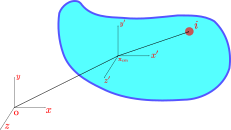
\includegraphics[width=0.7\textwidth]{images/rfc/images/rigid_body/rigid_body}
%   \caption{Body frame and local frame description of rigid body}
%   \label{fig:gloabl_body_frame_rb}
% \end{figure}
We use two coordinate frames to capture the dynamics of the rigid body, a
global frame and a body frame as shown in
\cref{fig:gloabl_body_frame_rb}. The body fixed frame, which moves with
rigid body is always located at the center of mass ($\ten{x}_{cm}$). The
state of the rigid body at a given time ($t$) can be described using position
($\ten{x}_{cm}$) and velocity ($\ten{v}_{cm}$) of the center of mass, a
rotation matrix($\ten{R}$) to represent the orientation of the rigid body with
respect to the global frame, and angular velocity($\teng{\omega}$). The center
of mass is computed as
\begin{equation}
  \label{eq:rfc:center_of_mass}
  \ten{x}_{cm} = \frac{\sum_i m_i \; \ten{x}_{i} }{\sum_i m_i }.
\end{equation}
The position of the discretized particle ($i$) in
\cref{fig:gloabl_body_frame_rb} belonging to the rigid body at time $t$ can be
computed as,
\begin{equation}
  \label{eq:rfc:rb_particle_pos_update}
  \ten{x}_i = \ten{x}_{cm} + \ten{r}_{i},
\end{equation}
with
\begin{equation}
  \label{eq:rfc:rb_particle_pos_update}
  \ten{r}_i = \ten{R} \overline{\ten{r}}_{i}.
\end{equation}
Here $\overline{\ten{r}}_{i}$ is the position of the particle $i$ about the body
frame axis and remains constant through out the simulation. The rotation matrix
$\ten{R}$ is used to bring the body frame position vector to the global frame
$\ten{O}$. Similarly the velocity vector is computed as,
\begin{equation}
  \label{eq:rfc:rb_particle_vel_update}
  \ten{v}_i = \ten{v}_{cm} + \teng{\omega} \times \ten{r}_{i}.
\end{equation}

We evolve the state of the rigid body through the integration of the
\cref{eq:rfc:balance_linear_mom,eq:rfc:balance_angular_mom}. The linear velocity of the
center of mass ($\ten{v}_{cm}$) and angular momentum ($\ten{L}$) at the next
timestep are computed as,
\begin{equation}
  \label{eq:rfc:lin_vel_cm_update}
  \ten{v}_{cm}^{n+1} = \ten{v}_{cm}^{n} + \frac{\ten{F}_{cm}}{M} \; \Delta t,
\end{equation}
\begin{equation}
  \label{eq:rfc:ang_mom_update}
  \ten{L}^{n+1} = \ten{L}^{n} + \teng{\tau}_{cm} \; \Delta t.
\end{equation}
Here, $\ten{F}_{cm} = \sum_i \ten{F}_i$.

The position of the center of mass and the rotation matrix ($\ten{R}$) are updated
by,
\begin{equation}
  \label{eq:rfc:lin_pos_cm_update}
  \ten{x}_{cm}^{n+1} = \ten{x}_{cm}^{n} + \ten{v}_{cm}^{n} \; \Delta t,\\
  \ten{R}^{n+1} = \ten{R}^{n} + \tilde{\teng{\omega}}^{n} \, \ten{R}^{n} \; \Delta t,
\end{equation}
where $\tilde{\teng{\omega}}^{n}$ is matrix formulation of angular velocity
$\omega$. The angular velocity at the new time step is computed with
\begin{equation}
  \label{eq:rfc:ang_velocity_update}
  \teng{\omega}^{n+1} = (\textit{\teng{I}}^{-1})^{n+1} \; \ten{L}^{n+1}.
\end{equation}
Here, moment of inertia at the new time step is computed as,
\begin{equation}
  \label{eq:rfc:moi_update}
  (\textit{\teng{I}}^{-1})^{n+1} = \ten{R}^{n+1} \textit{\teng{\overline{I}}}^{-1} (\ten{R}^{n+1})^T.
\end{equation}
where moment of inertia ($\textit{\teng{\overline{I}}}^{-1}$) in body frame is
used to compute in global frame at every time instant for faster computations.
The moment of inertia ($\textit{\teng{\overline{I}}}$) is computed as,
\begin{equation*}
\textit{\teng{\overline{I}}} =
\begin{bmatrix}
\sum_i m_i (y_i^2 + z_i^2) & -\sum_i m_i x_iy_i & -\sum_i m_i x_iz_i\\
-\sum_i m_i x_iy_i & \sum_i m_i (x_i^2 + z_i^2) &  -\sum_i m_i y_iz_i\\
-\sum_i m_i  x_iz_i & -\sum_i m_i y_iz_i & \sum_i m_i (x_i^2 + y_i^2)
\end{bmatrix}.
\end{equation*}

The position and velocity of the particles of the rigid body are updated by
\begin{eqnarray}
  \label{eq:rfc:rb_particle_pos_update}
  \ten{r}_i = \ten{R} \cdot \overline{\ten{r}}_{i},\\
  \ten{x}_i = \ten{x}_{cm} + \ten{r}_{i},\\
  \ten{v}_i = \ten{v}_{cm} + \teng{\omega} \times \ten{r}_{i}.
\end{eqnarray}

The force acting on particle $i$ is composed of interaction with the other rigid
bodies, and the fluid, given as
\begin{eqnarray}
  \label{eq:rfc:rb_particle_pos_update}
  \ten{F}_i = \ten{F}_{\text{Fl}}^i + \ten{F}_{\text{cont}}^i
\end{eqnarray}
We follow \cref{sec:contact-algorithm} to compute force
$\ten{F}_{\text{cont}}^a$ acting on particle $i$ due to the interaction with
the rigid bodies. The force $\ten{F}_{\text{Fl}}^i$ acting due to the
interaction with the fluid particles follows \cref{subsec:fsi}.

% We model the fluid with the CTVF \parencite{adepu2021corrected} scheme
developed in \cref{chap:ctvf}. Similar to the fluid modeling in
\cref{chap:fsi}, we modify the momentum equation to include the force acting due
to the interaction with a solid body. The discretized momentum equation of the
fluid particle including the interaction force is given as
\begin{multline}
  \label{eq:rfc:sph-momentum-fluid}
  \frac{\tilde{d}\ten{u}_{a}}{dt} = - \sum_{b} m_b \bigg[
  \bigg(\frac{p_a}{\rho_a^2} + \frac{p_b}{\rho_b^2}\bigg) \ten{I} -
  \bigg(\frac{\ten{A}_a}{\rho_a^2} + \frac{\ten{A}_b}{\rho_b^2}
  \bigg) \bigg]
  \cdot \nabla_{a} W_{ab} \\
  + \ten{u}_{a} \sum_{b} \frac{m_b}{\rho_{b}} \; \tilde{\ten{u}}_{ab} \cdot
  \nabla_{a} W_{ab} + \sum_{b} m_b \frac{4 \eta \nabla W_{ab}\cdot
    \ten{r}_{ab}}{(\rho_a + \rho_b) (r_{ab}^2 + 0.01 h_{ab}^2)} \ten{u}_{ab} +
  \ten{g}_{a} + \frac{\ten{F}^a_{\text{Fl}}}{m_a}.
\end{multline}
The particles are transported with a transport velocity as described in
\cref{chap:ctvf,chap:fsi}. The boundaries are handled using the dummy particle
approach as described in \cref{chap:ctvf}.

\subsection{Time Integration}

Rigid body and the fluid follow the kick-drift-kick time integration scheme. The
modeling of rigid-rigid interaction requires lower time step than the fluid. We
choose the minimum of both the timesteps to move the system forward in time. For
the numerical stability of fluid, the time step depends on the CFL condition as,
\begin{equation}
  \label{eq:rfc:time-step-cfl}
  \Delta t_{\text{fluid}} = \mathrm{min} \bigg( 0.25 \; \frac{h}{c + |U|} ,  0.25 \; \frac{h^2}{\nu},  0.25 \; \frac{h^2}{g} \bigg),
\end{equation}
where $|U|$ is the maximum velocity magnitude, $c$ is the speed of sound
typically chosen as $10 |U|$ for fluids in this work. For rigid body, the time
step is constrained as,
\begin{equation}
  \label{eq:rfc:time-step-body-force}
  \Delta t_{\text{rb}} \leq \frac{\pi}{50} \sqrt{\frac{m}{K_r}}.
\end{equation}
A minimum timestep is chosen as
\begin{equation}
  \label{eq:rfc:time-step-body-force}
  \Delta t = min(\Delta t_{\text{fluid}}, \Delta t_{\text{rb}}).
\end{equation}



\FloatBarrier%
\section{Discrete element method}
\label{sec:conclusions}





\FloatBarrier%
\section{Rigid fluid coupling}
\label{sec:conclusions}




\FloatBarrier%
\section{Results}
\label{sec:results}


\FloatBarrier%
\subsection{Stirrer in a fluid tank}
\label{sec:stirrer_fluid_result}


\FloatBarrier%
\subsection{Mixing of spherical particles in a tank}
\label{sec:stirrer_fluid_result}



\FloatBarrier%
\subsection{Mixing of spherical particles in a fluid tank}
\label{sec:mixing-spherical-particles-in-fluid-tank}



\FloatBarrier%
\section{Conclusions}
\label{sec:conclusions}


\section*{References}


\bibliographystyle{model6-num-names}
\bibliography{references}
\end{document}

% ============================
% Table template for reference
% ============================
% \begin{table}[!ht]
%   \centering
%   \begin{tabular}[!ht]{ll}
%     \toprule
%     Quantity & Values\\
%     \midrule
%     $L$, length of the domain & 1 m \\
%     Time of simulation & 2.5 s \\
%     $c_s$ & 10 m/s \\
%     $\rho_0$, reference density & 1 kg/m\textsuperscript{3} \\
%     Reynolds number & 200 \& 1000 \\
%     Resolution, $L/\Delta x_{\max} : L/\Delta x_{\min}$ & $[100:200]$ \& $[150:300]$\\
%     Smoothing length factor, $h/\Delta x$ & 1.0\\
%     \bottomrule
%   \end{tabular}
%   \caption{Parameters used for the Taylor-Green vortex problem.}%
%   \label{tab:tgv-params}
% \end{table}

%%% Local Variables:
%%% mode: latex
%%% TeX-master: "paper"
%%% fill-column: 78
%%% End:
